% !TEX TS-program = pdflatex


\documentclass{lncs/llncs}

\usepackage[T1]{fontenc}
%\usepackage{geometry}                % See geometry.pdf to learn the layout options. There are lots.
%\geometry{a4paper}                   % ... or a4paper or a5paper or ...
%\geometry{landscape}                % Activate for for rotated page geometry
%\usepackage[parfill]{parskip}    % Activate to begin paragraphs with an empty line rather than an indent
\usepackage{graphicx}

%\usepackage{amsfonts}
%\usepackage{fancyhdr}
%\usepackage{cite}
%\usepackage{ifthen}
%\usepackage{amssymb}
%\usepackage{fancyhdr}
%\usepackage{pifont}
\usepackage{stmaryrd}
\usepackage{mathtools,mathpartir}
\usepackage{proof}
%\usepackage{setspace}
%\usepackage{indentfirst}
\usepackage{amsmath,amssymb,amscd,mathrsfs}
\DeclareGraphicsRule{.tif}{png}{.png}{`convert #1 `dirname #1`/`basename #1 .tif`.png}
\usepackage{epsfig,color,subfigure,enumitem}
\newcommand{\TODO}[1]{\textcolor{red}{\textbf{[TODO:#1]}}}
\newcommand{\NOTE}[1]{\textcolor{blue}{\textbf{[NOTE:#1]}}}
\newcommand{\ERIC}[1]{\textcolor{blue}{#1}}
\newcommand{\coloncolon}{{:\hspace{-.2ex}:}}
\makeatletter
\newcommand{\raisemath}[1]{\mathpalette{\raisem@th{#1}}}
\newcommand{\raisem@th}[3]{\raisebox{#1}{$#2#3$}}
\makeatother

\usepackage{macrospNets}

\def\AlgT{\mathcal{T}}
\def\AlgE{\mathcal{E}}
\def\AlgA{\mathcal{A}}
\def\AlgAS{\mathcal{A}_S}
\def\AlgB{\mathcal{B}}
\def\AlgI{\mathcal{I}}

\newcommand{\Pred}{\symb{Pred}}
\newcommand{\Post}{\symb{Post}}
%\usepackage[math]{cellspace}
%\setlength\cellspacetoplimit{ 37pt}
%\setlength\cellspacebottomlimit{18pt}

\pagestyle{plain}

% addition to the mathpartir package for red dotted rules,
% that we use for open-transitions

\makeatletter
\def \dotover {\textcolor{red}{\leavevmode\cleaders\hb@xt@ .22em{\hss $\cdot$\hss}\hfill\kern\z@}}
\def \reddottedrule #1#2{\hbox {\advance \hsize by -0.5em
%\sbox0{$\genfrac{}{}{0pt}{0}{#1}{#2}$} \phantom{\copy0} %
 {\ooalign{\vphantom{$\genfrac{}{}{0pt}{0}{#1}{#2}$}\cr\dotover\cr$\genfrac{}{}{0pt}{0}{#1}{#2}$\cr}}}}

 \def \dottedrule #1#2 {
  {\sbox0{$\genfrac{}{}{0pt}{0}{#1}{#2}$}%
    \vphantom{\copy0}%
    \ooalign{%
      \hidewidth
      $\vcenter{\moveright\nulldelimiterspace
        \hbox to\wd0{%
         \xleaders\hbox{\kern.5pt\vrule height 0.4pt width 1.5pt\kern.5pt}\hfill
          \kern-1.5pt
        }%
      }$
      \hidewidth\cr
    \box0\cr}}
}

\let \defaultfraction \mpr@@fraction
\makeatother

%\newtheorem{theorem}{Theorem}[section]
\newtheorem{prop}[theorem]{Proposition}
%\newtheorem{corollary}[theorem]{Corollary}
%\newtheorem{lemma}[theorem]{Lemma}
\newtheorem{algorithm}[theorem]{Algorithm}
%\newtheorem{remark}[theorem]{Remark}
%\newtheorem{definition}[theorem]{Definition}
%\newtheorem{example}[theorem]{Example}
%\newtheorem{problem}[theorem]{Problem}
%\newtheorem{proof}[theorem]{Proof}

% Macros for the SOS rules and proof trees:
%\newcommand\openrule[2]{\redinfer{#1}{#2}}
\newcommand\openrule[2]{\inferrule*[myfraction=\reddottedrule,center]{#1}{#2}}
%\newcommand\openrule[2]{\inferrule*{#1}{#2}}
%\newcommand\ostate[1]{\triangleleft{\;#1\;}\triangleright}
\newcommand\ostate[1]{\triangleleft{#1}\triangleright}
\newcommand{\sm}[1]{\mbox{\boldmath\small #1}}



\title{Using SMT engine to generate Symbolic Automata\thanks{This work was partially 
funded by the Associated Team FM4CPS
  between INRIA and ECNU, Shanghai}}
\author{ Xudong Qin\inst{3}  \ \ \  Eric Madelaine\inst{1,2}} 
\institute{Univ. of Nice Sophia Antipolis, CNRS, UMR 7271, 06900 Sophia Antipolis, France
	\and INRIA Sophia Antipolis M\'edit\'erann\'ee, BP 93, 06902 Sophia Antipolis, France
\and Shanghai Key Laboratory of Trustworthy Computing, ECNU, China}
\date{}                                           % Activate to display a given date or no date

                          % Activate to display a given date or no date


\begin{document}

\maketitle

%\section{}
%\subsection{}


\begin{abstract}
  We implement the symbolic semantics of open pNets using their
  so-called ``Open Automaton'' behavioural semantics. This involve
  building predicates expressing the synchronisation conditions
  allowing some combination of events in the pNet system. These
  predicates are typically built using first order logic, plus some
  predicates specific of particular action algebras. To reduce the
  complexity of the generated open automata, we use the Z3 SMT engine
  to check satisfiability of the predicates, and prune the state
  space.. 

  

\end{abstract}


\section{Introduction}

\ERIC{imported from FORTE'16, }

In the nineties, several 
works extended the basic behavioural models based on labelled
transition systems to address value-passing or parameterised systems, using
various symbolic encodings of the
transitions~\cite{deSimone85,Larsen87,HennessyLin:TCS95,Linconcur96}. 
In \cite{Linconcur96}, H.M. Lin addressed value-passing calculi, for which he
developed a symbolic behavioural semantics, and proved algebraic properties.
Separately J. Rathke~\cite{HennessyRathke:TCS98} defined another
symbolic semantics for 
a parameterised broadcast calculus, together with strong and weak bisimulation
equivalences, and developed a symbolic model-checker based on a tableau
method for these processes. 30 years later, no
practical verification approach and no verification platform are
using this kind of approaches to provide proof methods for
value-passing processes or open process expressions. 

\paragraph{Context}
\TODO{
  Summary of previous works on pNets and open pNets => 1/2 page.\\
  Longterm goals:\\
  - open pNets to represent operators and program skeletons (ref to
  \cite{PDP2015})\\
  - compute semantics in term of open transitions\\
  - compute equivalence (bisimulation of open automata)\\
  - model-check properties of open systems
  }
\paragraph{Contribution}

\paragraph{Related works}



\paragraph{Structure.}

\section{Running Example(s)}

\section{Parameterised Networks (pNets): definition}
\label{section:pnets}

\ERIC{Keep minimum defs here too be independent from FORTE}

This section introduces pNets and the notations we will use in
this paper. Then it gives the formal definition of pNet structures,
together with an operational semantics for open pNets.

pNets are tree-like structures, where the leaves are either
\emph{parameterised labelled transition systems (pLTSs)}, expressing the
behaviour of basic processes, or \emph{holes}, used as placeholders
for unknown processes, of which we only specify the set of possible
actions, this set is named the \emph{sort}.
Nodes of the tree (pNet nodes) are synchronising artifacts, using a
set of \emph{synchronisation vectors} that express the possible
synchronisation between the parameterised actions of a subset of the
sub-trees.


%\smallskip\noindent
\paragraph*{Notations.}
We extensively use indexed structures
over some countable indexed sets, which are equivalent to mappings over
the countable set. % . The indexes will usually be
% integers, bounded or not. Such an indexed family is
%denoted
%follows:
$a_i^{i\in I}$
%, or equivalently  $(i\mapsto a_i)^{i\in I}$
denotes a family of elements $a_i$ indexed over the
set $I$. % Such a family
% is equivalent to the mapping $(i\mapsto a_i)^{i\in I}$.
% To specify the set over which the structure is indexed,
% indexed structures are always denoted with an exponent of the form $i\in I$
% (arithmetic only appears in the indexes if necessary).
$a_i^{i\in I}$ defines both $I$ the set over which the family is
indexed (called \emph{range}), and $a_i$ the elements of the family.
E.g., $a^{i\in\{3\}}$ is the mapping with a single entry $a$ at index
$3$ ; abbreviated $(3\mapsto a)$ in the following.
When this is not
ambiguous, we shall use notations for sets, and typically write
``indexed set over I'' when formally we should speak of multisets, and
write $x\in a_i^{i\in I}$ to mean $\exists i\in I.\, x=a_i$.  An empty
family is denoted $\emptyset$. We
denote classically $\overline{a}$ a family when the indexing set is
not meaningful.  $\uplus$ is the disjoint union on
indexed sets.


\paragraph*{Term algebra.}
Our models rely on a notion of parameterised actions, that are
symbolic expressions using data types and variables. As our model aims
at encoding the low-level behaviour of possibly very different
programming languages, we do not want to impose one specific algebra
for denoting actions, nor any specific communication mechanism. So we
leave unspecified the constructors of the algebra that will allow building
expressions and actions. Moreover, we use a generic {\em action interaction}
mechanism, based on (some sort of) unification between two or more action
expressions, to express various kinds of communication or
synchronisation mechanisms.

\def\Talg{\mathcal{T}_{\Sigma,\P}}
Formally, we assume the existence of a term algebra $\Talg$,
where $\Sigma$ is the signature of the data and action constructors,
and $\P$ a set of variables. Within $\Talg$, we distinguish a set of
data expressions $\mathcal{E}_\P$, including a set of boolean
expressions $\mathcal{B}_{\P}$ ($\mathcal{B}_{\P}\subseteq\mathcal{E}_\P$).
On top of $\mathcal{E}_\P$ we build the action algebra
$\mathcal{A}_\P$, with $\mathcal{A}_P\subseteq\mathcal{T}_\P,
\mathcal{E}_P\cap\mathcal{A}_P=\emptyset$;
naturally action terms will use data expressions as subterms.
To be able to reason about the data flow between pLTSs, we
distinguish \emph{input variables} of the form $?x$ within terms; the function
$\vars(t)$ identifies the set of variables in a term
$t\in\AlgT$, and $iv(t)$ returns its input variables.


pNets can encode naturally the notion of input actions in value-passing CCS
\cite{Milner89} or of usual point-to-point message passing calculi, but it also allows
for more general mechanisms, like gate negociation in Lotos, or broadcast
communications. Using our notations, value-passing actions \emph{\`a la} CCS would be
encoded as $a(?x_1,...,?x_n)$ for inputs, $a(v_1,..,v_n)$ for outputs (in which $v_i$ are 
action terms containing no input variables). 
%For Lotos-style
%distributed synchronisation, we use synchronisation vectors that encode matching data
%offers on a common gate; or 
We can also use more complex action structure such as Meije-SCCS action
monoids, like in $a.b$, $a^{f(n)}$ (see \cite{deSimone85}). The expressiveness of the synchronisation constructs
will depend on the action algebra.




\subsection{The (open) pNets Core Model}
\label{section:pNets}


A pLTS is a labelled transition system with variables; variables can be
manipulated, defined, or accessed inside states, actions, guards, and
assignments. Without loss of generality and to simplify the formalisation, we suppose 
here that 
variables are local to each 
state: each state has its set of variables disjoint from the others. Transmitting 
variable values from one state to the other can be done by explicit assignment. 
%Similarly, to simplify the management of variables and without loss of expressivity, we 
%suppose that transitions looping to the same state does not do assignments.
Note that we make no assumption on finiteness of the set of states nor
on finite branching of the transition relation.

We first define the set of actions a pLTS can use, let $a$
range over action labels, $\symb{op}$ are operators, and $x_i$ range over
variable names. Action terms are:
\[
\begin{array}[l]{rcl@{\quad}p{5.5cm}}
  \alpha\in\AlgA&::=&a(p_1,\ldots,p_n)&\text{action terms}\\
  p_i&::=& ?x~|~\symb{Expr}&\text{parameters (input variable or expression)}\\
  \symb{Expr}&::=& \symb{Value}~|~x~|~\symb{op}(\symb{Expr}_1,..,\symb{Expr}_n)&\text{Expressions}
\end{array}
\]
The input variables in an action term are those marked with a
$\symb{?}$.
We additionally suppose that each input variable does not
appear somewhere else in the same action term:
$p_i=?x\Rightarrow\forall j\neq i.\, x\notin \vars(p_j)$

\begin{definition}[pLTS]
\label{pLTS}
A pLTS is a tuple
$pLTS\triangleq\mylangle S,s_0, \to\myrangle$ where:
\begin{itemize}
\item[$\bullet$]
$S$ is a set of states.
\item[$\bullet$]
$s_0 \in S$ is the initial state.
%\item[$\bullet$]
 %Variables in
%$\iv(\alpha)$ are assigned by the action, other variables can be assigned
%by the additional assignments.
\item[$\bullet$] $\to \subseteq S \times L \times S$ is the transition relation and 
$L$ is the set of labels of the form
$\langle \alpha,~e_b,~(x_j\!:= {e}_j)^{j\in J}\rangle$,
where $\alpha \in\AlgA$ is a parameterised action, $e_b \in
\AlgB$ is a guard, and the variables $x_j\in P$
are assigned the expressions $e_j\in \AlgE$.
If 
$s \xrightarrow{\langle \alpha,~e_b,~(x_j\!:= {e}_j)^{j\in
		J}\rangle} s'\in \to $ then $\iv(\alpha)\!\subseteq\! \vars(s')$, 
		$\vars(\alpha)\backslash \iv(\alpha)\!\subseteq\! \vars(s)$, 
		$\vars(e_b)\!\subseteq\! \vars(s')$, and
		$\forall j\!\in\! J .\,\vars(e_j)\!\subseteq\! \vars(s)\land 
		x_j\!\in\!\vars(s')$. %,  and $s= s'\Rightarrow J=\emptyset$. 
		
\end{itemize}
\end{definition}

Now we define
pNet nodes, as constructors for hierarchical behavioural structures.
A pNet has a set of sub-pNets that can be either pNets or pLTSs, and a
set of Holes, playing the role of process parameters.

A composite pNet consists of a set of sub-pNets exposing
a set of actions, each of them triggering internal actions in each of
the sub-pNets. The synchronisation between global actions and
internal actions is given by  \emph{synchronisation vectors}: a
synchronisation vector synchronises one or several internal actions, and
exposes a single resulting global action.
Actions involved at the pNet level (in the synchronisation vectors) do
not need to distinguish between input and output
variables. Action terms for pNets are defined as follows:
\[\begin{array}[l]{rcl@{\quad}l}
  \alpha\in \AlgAS &::=&a(Expr_1,\ldots,Expr_n)
\end{array}
\]



\begin{definition}[pNets]\label{def-pnets}
A pNet is a hierarchical structure where leaves are pLTSs and holes:\\
$\pNet\triangleq pLTS~|~\mylangle \pNet_i^{i\in I}, S_j^{j\in J}, \symb{SV}_k^{k\in K}\myrangle$
where
\begin{itemize}
\item[$\bullet$] $I \in \I$ is the set over which sub-pNets are indexed.
\item[$\bullet$] $\pNet_i^{i\in I}$ is the family of sub-pNets.
%  $\pNet_i^{i\in I}$ is a family of sub-pNets where $I\in\I_\P$ is the set over which sub-pNets are indexed.

\item[$\bullet$] $J\in\I_\P$ is the set over which holes are indexed.
$I$ and $J$ are \emph{disjoint}: $I\cap J=\emptyset$,  $I\cup J\neq\emptyset$
\item[$\bullet$] $S_j \subseteq \AlgAS$ is a set of action terms, denoting the $\Sort$ of
hole $j$.

\item[$\bullet$] $\symb{SV}_k^{k\in K}$ is a set of
  synchronisation vectors ($K\in\I_\P$). $\forall k\!\in\! K,
  \symb{SV}_k\!=\!\alpha_{l}^{l\in I_k \uplus J_k}\to\alpha'_k$ where
  $\alpha'_k\in \mathcal{A}_\P$, $I_k\subseteq I$, $J_k\subseteq J$,
  $\forall i\!\in\!
  I_k.\,\alpha_{i}\!\in\!\Sort(\pNet_i)$,  $\forall j\!\in\!
  J_k.\,\alpha_{j}\!\in\!S_j$, and $\vars(\alpha'_k)\subseteq \bigcup_{l\in I_k\uplus 
  J_k}{\vars({\alpha_l})}$. The global action of a vector $\symb{SV}_k$ is
$\Label(\symb{SV}_k) = \alpha'_k$.


\end{itemize}
\end{definition}

The preceding definition relies on the auxiliary functions below:

\begin{definition}[Sorts, Holes, Leaves of pNets]
  \begin{itemize}
  \item The sort of a pNet is its signature, i.e. the set of actions it can
perform. In the definition of sorts, we do not need to distinguish
input variables (that specify the dataflow within LTSs), so for
computing LTS sorts, we use a substitution operator\footnote{$\subst{y_k\gets x_k}^{k\in K}$ is the parallel substitution 
operation.} to remove the
\emph{input marker} of variables. Formally:
\[
\begin{array}{l}
\Sort(\mylangle S,s_0, \to\myrangle) = \{\alpha\subst{x \gets ?x| 
x\in\symb{iv}(\alpha)}|s \xrightarrow{\langle \alpha,~e_b,~(x_j\!:= {e}_j)^{j\in
		J}\rangle} s'\in \to \} \\ \Sort(\mylangle
\set{\pNet}, \set{\symb{S}}, \set{\symb{SV}}\myrangle) =\{\alpha'_k |\, \alpha_j^{j\in J_k}\to\alpha'_k\in\set{\symb{SV}}\}
\end{array}
\]

\item
The set of holes of a pNet is defined inductively; the sets of holes
in a pNet node and its subnets are all disjoint:
  \[\begin{array}{l}
\Holes(\mylangle S,s_0, \to\myrangle) \!=\! \emptyset \\
\Holes(\mylangle \pNet_i^{i\in I}\!,S_j^{j\in J}\!, \overline{\symb{SV}}\myrangle) =J\cup{\displaystyle \bigcup_{i\in I}\Holes(\pNet_i)}\\
\forall i\in I.\, \Holes(\pNet_i)\cap J=\emptyset\\
\forall i_1,i_2\in I.\,i_1\neq i_2\Rightarrow  \Holes(\pNet_{i_1})\cap\Holes(\pNet_{i_2})=\emptyset
\end{array}\]
\item
The set of leaves of a pNet is the set of all pLTSs occurring in the structure, defined inductively as:
\[\begin{array}{l}
\Leaves(\mylangle S,s_0, \to\myrangle) \!=\! \{ \mylangle S,s_0, \to\myrangle \}\\
\Leaves(\mylangle \pNet_i^{i\in I}\!,S_j^{j\in J}\!, \overline{\symb{SV}}\myrangle) = {\displaystyle \bigcup_{i\in I}\Leaves(\pNet_i)}
\end{array}\]
\end{itemize}
\end{definition}

A pNet $Q$ is \emph{closed} if it has no hole: $\Holes(Q)=\emptyset$; else it
is said to be \emph{open}.


\begin{figure}[t]
\begin{minipage}{6.1cm}

  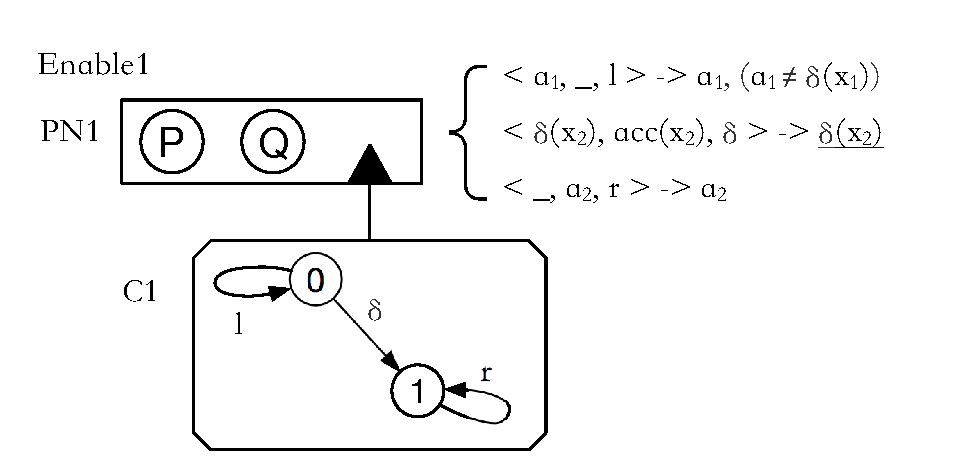
\includegraphics[width=\linewidth]{XFIG/Enable1}
  \\[1.3ex]
 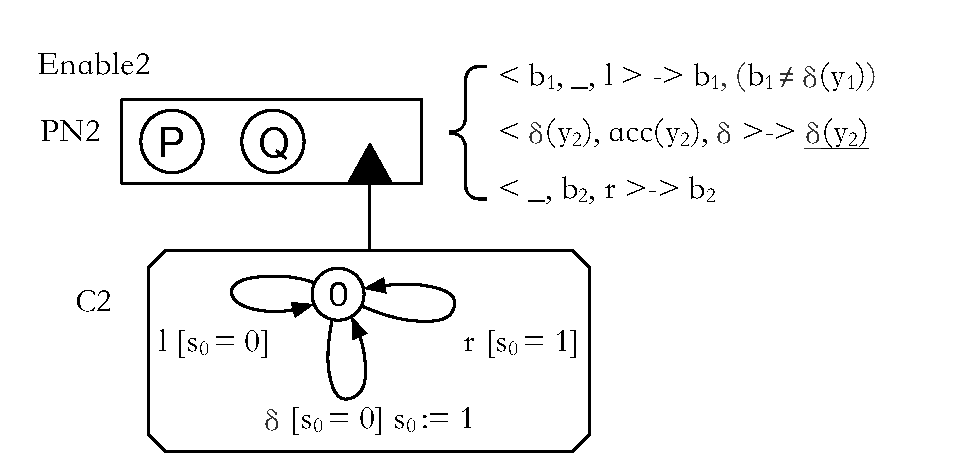
\includegraphics[width=\linewidth]{XFIG/Enable2}
  \caption{Two pNet encodings for  Enable }  \label{schema:enable-pnets}
\end{minipage}
  \hspace{2mm}
\begin{minipage}{6cm}
  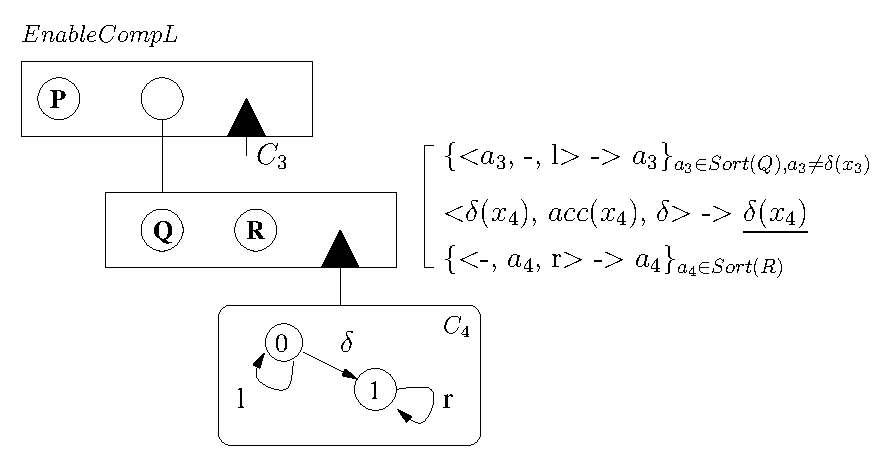
\includegraphics[width=\linewidth]{XFIG/P-QR}
  \caption{Composed pNet for ``P>>(Q>>R)''}  \label{schema:enable-composed}
\end{minipage}

\end{figure}





\section{Operational Semantics for Open pNets}
\label{section:op-semantics}



The semantics of open pNets will be defined  as an open automaton. An open
automaton is an automaton where each transition composes transitions of several LTSs with
action of some holes, the transition occurs if some predicates hold, and can involve a 
set of state modifications.

\begin{definition}[Open transitions]
	\label{def:OpenTransitions}
	An \emph{open transition} over a set  $(S_i,s_{0 i}, \rightarrow_i)^{i\in
	I}$ of LTSs, a
	set $J$ of holes with sorts $Sort_j^{j\in J}$, and a set of states $\mathcal{S}$ is a structure of the form:	
	\begin{mathpar}
	\inferrule*[myfraction=\reddottedrule]
	{\{s_i~{\xrightarrow{a_i}}_i ~s_i^{\prime}\}^{i\in I},
		\{\xrightarrow{b_j}_j\}^{j\in J}, \Pred, \Post}
	{s \xrightarrow {v}s'}
	\end{mathpar}
	Where $s, s'\in\mathcal{S}$ and for all
        $i\in I$, $s_i{\xrightarrow{a_i}}_i s_i^{\prime}$ is a transition of the
	LTS $(S_i,s_{0 i}, \rightarrow_i)$, and $\xrightarrow{b_j}_j$
        is a transition of the hole $j$, for any action $b_j$ in the
        sort $Sort_j$. \Pred\ is a predicate
	over the different variables of the
	terms, labels, and states $s_i$, $b_j$, $s$, $v$. \Post\ is a set of equations that 
	hold \emph{after the open transition}, they are represented as a substitution of the 
	form $\{x_k\gets e_k\}^{k\in K}$ 
	where $x_k$ are variables of $s'$, $s'_i$, and $e_k$ are expressions over the other 
	variables of the open transition.
\end{definition}

\begin{example}\emph{An open-transition.}
  \label{OT:enable-composed}
  The \texttt{EnableCompL} pNet of Fig. \ref{schema:enable-composed} has 2 controllers and 2 holes. One of its possible open-transition is:

 \smallskip
 $  OT_2  = \openrule{
                       0 \xrightarrow{\delta}_{C_3} 1 ~~
                            0 \xrightarrow{l}_{C_4} 0  ~~                 
                            \xrightarrow{\delta(x4)}_P ~~
                            \xrightarrow{accept(x4)}_Q 
                      }
  %  {\ostate{00} \xrightarrow{\underline{\delta(x1)}} \ostate{10}}
    {A1_0 \xrightarrow{\underline{\delta(x4)}} A1_1}
  $
\end{example}


\begin{definition}[Open automaton]
	\label{def:open-automaton}
	An \emph{open automaton} is a structure\\ $A =
	<LTS_i^{i\in I},J,\mathcal{S},s_0,\mathcal{T}>$ where:
	\begin{itemize}
		\item[$\bullet$]  $I$ and $J$ are  sets of indices,
		\item[$\bullet$]  $LTS_i^{i\in I}$ is a family of LTSs,
		\item[$\bullet$]   $\mathcal{S}$ is a set of states and $s_0$ an initial state
		among $\mathcal{S}$,
		\item[$\bullet$] $\mathcal{T}$ is a set of open transitions and for each
		$t\in \mathcal{T}$ there exist $I'$, $J'$ with $I'\subseteq I$, $J'
		\subseteq J$, such that $t$ is an open transition over $LTS_i^{i\in I'}$, $J'$,
		and  $\mathcal{S}$.
		
	\end{itemize}
\end{definition}
	

%
%Then the semantics of a pNet is characterized by a set of {\em open
%transitions}, where the hypotheses on process parameters are
%replaced by 1) transitions of the pLTSs at the leaves, and 2) formal
%hypotheses on the transitions of the holes. A {\em predicate} is used
%to relate the parameters and names appearing in the actions of the
%leaves and the holes involved in the rules, but also appearing in  the resulting action.


\begin{definition}[States of open pNets]\label{def-states}
  A state of an open pNet is a tuple (not necessarily finite) of the
  states of its leaves (in which we denote tuples
  in structured states as $\triangleleft\ldots\triangleright$ for better readability).

  For any pNet p, let $\overline{Leaves} = \mylangle S_i,{s_i}_0, \to_i\myrangle^{i \in L}$ be the set of pLTS at its leaves,
  then $States(p) = \{\triangleleft s_i^{i\in L}
  \triangleright| \forall i\in L. s_i \in S_i\}$.
A pLTS being its own single leave:
  $States(\mylangle S,s_0, \to\myrangle) = \{\triangleleft s \triangleright| s \in S\}$.

The initial state is defined as:
$InitState(p) = \triangleleft {{s_i}_0}^{i\in L}  \triangleright$.
\end{definition}

%% \begin{example} \emph{State of a pNet}
%%   The states of pNet \texttt{EnableCompL} are:
%%   $\triangleleft 00 \triangleright, \triangleleft 10 \triangleright, \triangleleft 11 \triangleright$
%% \end{example}

\paragraph{Predicates:}
Let
$\mylangle\overline{\pNet},\overline{S},\symb{SV}_k^{k\in K} \myrangle$
be a pNet. Consider a synchronisation vector $SV_k$, for $k\in K$. We define a
predicate $\Pred$ relating
the actions of the involved sub-pNets and the resulting actions. This predicate verifies:
\[\Pred(SV_k, a_i^{i\in I}, b_j^{j\in J}, v)\Leftrightarrow
\begin{array}{l}
\exists {(a'_i)}^{i\in I},
{(b'_j)}^{j\in J},v'.\, SV_k={(a'_i)}^{i\in I}, {(b'_j)}^{j\in J}\rightarrow v'
\\~~\land
\forall i\in I.\, a_i=a'_i\land \forall j \in J.\, b_j=b'_j \land v=v'
\end{array}\]
In any other case (if the action families do not match or if there is no valuation of
variables such that the above formula can be ensured) the predicate is undefined.

This definition is not constructive but it is easy to build the predicate constructively
by brute-force unification of the sub-pNets
actions with the corresponding vector actions, possibly followed by a simplification
step.


We build the semantics of open pNets as an open automaton where LTSs are the pLTSs at
the leaves of the pNet structure, and the states are given by 
Definition~\ref{def-states}. The open transitions first
 project the global state into states of the leaves, then apply
pLTS transitions on these states, and compose them with the sort of the holes. %The pNet
%structure does not appear in the open-automaton, only the
%set of Holes and the set of Leaves.
The semantics   regularly instantiates \emph{fresh} variables, and uses a
\emph{clone} operator that clones a term replacing each variable with a
fresh one.

\begin{definition}[Operational semantics of open pNets]
	\label{def:operationalSemantics}
	The semantics of a pNet $p$ is an open automaton $A = <Leaves(p),J,\mathcal{S}, s_0,
	\mathcal{T}>$ where:
	\begin{itemize}
		\item $J$ is the indices of the holes: $Holes(p)= H_j^{j\in J}$.
		%  \item $\overline{L}^L = Leaves(p), \overline{H}^J = Holes(p)$
		\item $\overline{\mathcal{S}} = States(p)$ and $s_0 = InitState(p)$
		\item $\mathcal{T}$ is the smallest set of open transitions
		satisfying the rules below:
	\end{itemize}
	
	
	The rule for a pLTS $p$  checks that the guard 
	is verified and transforms assignments into post-conditions:
	
	\begin{description}
		\item[{\bf Tr1:}]
		$\inferrule
		{ s \xrightarrow{\langle \alpha,~e_b,~(x_j\!:= {e}_j)^{j\in
					J}\rangle} s'\in \to  }
		{ p = \mylangle  S,s_0, \to \myrangle
			\models
			\inferrule*[myfraction=\reddottedrule]
			{\{s \xrightarrow{\alpha}_p s'\} ,\emptyset ,
			e_b,\left\{x_j\gets e_j\right\}^{j\in J}}
			{\ostate{s} \xrightarrow{\alpha} \ostate{s'}}
		}
		$
	\end{description}
%	Note that this note is greatly simplified by the fact that variables are local to 
%	thread; introducing global state variables or accepting loops to the same 
%	state would 
%	require to reason 
%	on the scope of 
%	each variables, and to introduce additional variables to handle the several occurence 
%	of the same pLTS variable in the predicates. Indeed the constraints on pLTS 
%	transitions 
%	ensure that the same variable never appears both on the left and on the right of the 
%	equations of a predicate.
	
	The second rule deals with pNet nodes: for each possible
	synchronisation vector applicable to the rule subject, the premisses
	include one {\em open transition} for each sub-pNet involved, one possible
	{\em action} for each Hole involved, and the predicate relating these
	with the resulting action of the vector.
	A key to understand this rule is that the open transitions are
	expressed in terms of the leaves and holes of the pNet structure,
	i.e. a flatten view of the pNet: e.g. $L$ is the index set of the
	Leaves, $L_k$ the index set of the leaves of one subnet, so all $L_k$
	are disjoint subsets of $L$. Thus the states in the open transitions,
	at each level, are tuples including states of all the
	leaves of the pNet, not only those involved in the chosen
	synchronisation vector.
	
	\begin{description}
		\item[{\bf Tr2:}]
	\end{description}
	
	\noindent
    $\inferrule
    {k\!\in\! K \\ SV\!\!= \!clone(SV_k) \!=\! \alpha_m^{m \in I_k\uplus J_k} \!\to\! 
    \alpha'_k \\
    	Leaves(p) \!=\! \pLTS_l^{l\in L} \\    	
    	\forall m\in I_k.
    	\pNet_m \models
    	\inferrule*[myfraction=\reddottedrule]
    	{\{s_{i}\xrightarrow{a_{i}}_i s_{i}'\}^{i\in I_m^\prime},
    	\{\xrightarrow{b_{j}}_j\}^{j\in J'_m}, \Pred_m, \Post_m}
    	{\ostate{s_{i}^{i \in L_m}} \xrightarrow {v_m}
    		\ostate{s_{i}^{\prime\ i \in L_m}}}
    	%\land
    	%Leaves(\pNet_m) = \overline{pLTS}^{L_k})
    	\\
    	I' = \biguplus_{m\in I_k}\!\! I_m'
    	\\ J' = \biguplus_{m\in I_k}\!\! J'_m \uplus J_k 	\\
    	\Pred = \bigwedge_{m\in I_k}\!\! \Pred_m \land
    	\Pred(SV,a_i^{i\in I_k},b_j^{j\in J_k},v)\\
    	\forall j\!\!\in\!\! J_k. {\tt 
    		fresh}(b_j) \\ {\tt fresh}(v) \\ 
    	\forall i\in
    	L\backslash I'.\,s'_i=s_i 
    }
    {p = \mylangle \pNet_i^{i\in I}, S_j^{j\in J}, \symb{SV}_k^{k\in K}\myrangle
    	\models
    	{\inferrule*[myfraction=\reddottedrule]
    		{\{s_i\xrightarrow{a_i}_i s_i^{\prime}\}^{i\in I^\prime},
    		\{\xrightarrow{b_j}_j\}^{j\in J^\prime}, \Pred, \uplus_{m\in I_k} 
    		\Post_m}
    		{\ostate{s_i^{i\in L}} \xrightarrow {v}
    			\ostate{s_i^{\prime i\in L}}}
    	}
    }
    $
	



	
	\medskip
	
\end{definition}
%

\begin{example} \emph{Using the operational rules to compute
    open-transitions}
  In Fig. \ref{usingrules:OT2} we show the deduction tree used to construct and prove the 
  open transition $OT_2$ of \texttt{EnableCompL} (see example page \pageref{OT:enable-composed}).
  The rule uses TR1 for the $\delta$ transition of $C_3$, for the $l$ transition of $C_4$, then combines the result using the $a_4$ vector of the bottom pNet node, and the $\underline{\delta(x)}$ vector of the top node.
  
\begin{figure}[tb]
\begin{mathpar}
  \small
  \inferrule
    {\inferrule
        {0 \xrightarrow {\delta}_{C_3} 1}
        {C_3
          \models
            \openrule{
              0 \xrightarrow {\delta}_{C_3} 1,\,
              \{\xrightarrow{\delta(x_1)}_P\},\,
              v_1=\delta(x_1)}
                      {\ostate{0}\xrightarrow{v_1}\ostate{1}}
        }\\
%      \sm{fresh}v         \\
      \inferrule%*[right={L_1}]
        {
%          \sm{fresh}{a_Q} \\
          \inferrule
              {0 \xrightarrow{l}_{C_4} 0}
              % {\ostate{0}\xrightarrow{l}\ostate{0}}
              {C_4
                \models
                \openrule{
                      0 \xrightarrow l_{C_4} 0,\,
                      \sm{Pred}_{C_4}}
                      {\ostate{0}\xrightarrow{l}\ostate{0}}
              }
        }
        {
          \textrm{Q>>R}\models
              \openrule
                  { 0 \xrightarrow {l}_{C_4} 0,\,
                    \{\xrightarrow{acc(x_2)}_Q\},\,
                    \ v_2=acc(x_2)
                  }
                  {\ostate{0}\xrightarrow{v_2}\ostate{0}}
        }   
    }
    {
     \textrm{P>>(Q>>R)}
     \models
     \openrule
         { 0 \xrightarrow{\delta}_{C_3} 1, \\ 0 \xrightarrow{l}_{C_4} 0,\\
           \{\xrightarrow{\delta(x)}_P,\,\xrightarrow{acc(x)}_Q\}, \\
            a_3=v_1 \wedge v=a_3 \wedge x_1=x_2
           }
         {\ostate{00} \xrightarrow{v} \ostate{10}}
      }\vspace{-4ex}
\end{mathpar}
  \caption{Proof of transition $OT_2$ (with interaction of processes $P$ and $Q$) for ``P>>(Q>>R)''}
  \label{usingrules:OT2}
\end{figure}

\end{example}

    

Note that while the scenario above is expressed as a single
instantiation of the possible behaviours, the constructions below are
kept symbolic, and each open-transition deduced expresses a whole family of
behaviours, for any possible values of the variables.

\paragraph{Variable management.}
The variables in each synchronisation vector are considered local:
for a given pNet expression, we must have fresh local variables for
each occurrence of a vector (= each time we instantiate rule
Tr2). Similarly the state variables of each copy of a
given pLTS in the system, must be distinct, and those created for each
application of Tr2 have to be fresh and all distinct. 
This will be implemented within the open-automaton generation algorithm,
e.g. using name generation using a global counter as a suffix.


\subsection{Computing and using open automata}
In this section we present an algorithm to construct the open
automaton representing the behaviour of an open pNet, and we prove that
under reasonable conditions this automaton is finite.

\TODO{Refine the algorithm description}

\begin{algorithm}[Behavioural semantics of open pNets: Sketch]
This is a standard residual algorithm over a set of open-automaton
states, but where transitions are open transitions
constructively ``proven'' by deduction trees.

1) Start with a set of unexplored states containing the initial state
of the automaton, and an empty set of explored states.

2) While there are unexplored states:

2a) pick one state from the unexplored set and add it to the explored
set. From this state
build all possible deduction trees by application of the structural
rules Tr1 and Tr2, using all \ERIC{applicable} combinations
of synchronisation vectors.

2b) For each of the obtained deduction trees, extract the resulting
open-transition, with its predicate and \Post\ assignments by exploring the structure of 
the pNet.

2c)
\ERIC{The predicate is submitted to Z3 for checking satisfiability. If it is NOT stisfiable, the resulting OT is discarded. This will minimize the number of
resulting transitions, and potentialy prune the search-space.}

2d)
\ERIC{Optionally, simplify the predicate by eliminating the unnecessary intermediate variables, that were produced as fresh local variables of synchronisation vectors, and fresh result variables of intermediate OTs. In the resulting predicate the only significant variables are :\\
- the input variables of pLTS transitions\\
- the actions of holes\\
- the result action at toplevel.}

For each open-transition,  add the transition in the outgoing transitions of
the current state, and add the
resulting state in the unexplored set if it is not already in the
explored set.

%3) this ends with the "while" from step 2, when we have no more
%unexplored set.
\end{algorithm}



To have some practical interest, it is important to know when this
algorithm terminates. The following theorem shows that an open-pNet
with finite synchronisation sets, finitely many leaves and
holes, and each pLTS at leaves having a finite number of states and
(symbolic) transitions, has a finite automaton:

\begin{theorem}[Finiteness of open-automata.]\\
Given an open pNet $\mylangle \overline{\pNet},\overline{S}, \symb{SV}_k^{k\in K}\myrangle$ with leaves $pLTS_i^{i\in L}$ and holes $Hole_j^{j\in
  J}$, if the sets $L$ and $J$ are finite, if the synchronisation vectors of all pNets 
  included in  $\mylangle \overline{\pNet},\overline{S}, \symb{SV}_k^{k\in K}\myrangle$ 
  are finite, and if
$\forall i \in L.\, finite{(states(pLTS_i))} \text{ and } pLTS_i$
has a finite number of state variables, then Algorithm 1 terminates
and produces an open automaton 
$\mathcal{T}$ with finitely many states and transitions.


% Given an open pNet $\mylangle \overline{\pNet},\overline{S}, \symb{SV}_k^{k\in
%     K}\myrangle$ with leaves $pLTS_i^{i\in L}$ and holes $Hole_j^{j\in
%   J}$,
% build its semantics as in algorithm 1.

% We have:

% $$ finite{(L)} \land finite{(J)} \land \forall i \in L finite{(\{s_i\})}
%   \to finite{(\mathcal{T})}$$
\end{theorem}

\section{Implementation}

\TODO{
Xudong: Detailed description of the implementation\\\\
5.1 Generation of the Open Transition\\\\
5.1.1 fresh variable\\\\
The variable in each SV are considered local, so does the variable of an open transition such as its hole behavior and its result action.
So we want rename them to make them unique, while we also hope them readable. The fresh variable has a confirmed format.
As pNets has a tree-like structure, we give every node of the pNets a tree index. And give them some counters to count the current times the SV, Hole or subnet is used, and the number of possible OT generated. \\\\
| format of fresh variable |\\\\
5.1.2 predicate generation\\\\
Combining, present all the possible working status of subnets. \\
Mixing, match the elements of the combination to match the elements of the SV one by one to generate terms of a predicate.\\\\
5.1.3 assignment\\\\
Management of state variables.\\
Translating assignments into predicate terms.\\\\
5.2 Pruning the unsatisfiable results\\\\
Interaction with Z3: pNets module ---input--> Z3 module [JAVA API]\\\\
5.2.1 presentation\\\\
5.2.2 checking satisfiability\\\\
After we get the result OTs, for each result OT, declare the variables and assertions in the Java API. Conduct checking method and get the result.\\
}

\ERIC{
=> Context VCE, ref to FASE paper\\
=> Current prototype: programatic creation of pNet objects, through the pNet API in VCE. On the middle term, this should be compiled from some language or graphical formalism.\\
=> Open transitions are computed as a direct implementation of the algorithm above. Steps 2a-2b are merged: at each pNet node, after application of rule Tr2, the resulting OT is built from the premisses, without explicitely constructing the deduction tree. \\
=> Variable names are generated for all ``fresh'' and ``clone''
operations, using structured variable names ensuring uniqueness of
fresh names, but also reasonable readability of these names for
debugging purposes.\\
=> Assignements\\
=> Satisfiability check is done only at toplevel of the deduction tree construction. An alternative would be to submit the satisfiability check to the SMT solver at each level of the tree construction, potentialy reducing the overall number of combinations. But submission to the SMT engine is costly, and more complexity analysis is required before deciding if this would be worthwhile.\\
=> Simplification is not yet implemented. It is not strictly required for the Open Automaton construction, but it will be critical later for predicate comparison in the bisimulation algorithm.}


\TODO{
Xudong: full result of the tool execution on the running example\\\\
Open Automata of the CCS example.
}




\section{Conclusion and Discussion}
\label{section:conclusion}


  

\bibliographystyle{lncs/splncs}

% \bibliography{oasis,biblio}
\bibliography{biblio}

% \newpage
% \appendix

\end{document}
